\section{What does the first principal component capture?}
We have described the score in the first principal component as a proxy for diversity of the export basket, where products are weighted by their complexity or sophistication. We explore here more in detail what this first component captures.

From the definition of what PCA does, we know that the first principal component $\scoreFirstPC$ captures the largest amount of variability across export baskets (the latter transformed using our measure $R_{cpt}$ of scaled absolute advantage). As shown before, the first principal component explains almost sixty percent of the variance, and the loadings of the vector are positive and approximately of the same magnitude. This necessarily means that the scores in this $\scoreFirstPC$ must capture an \emph{average scaled absolute advantage}. Given the formula of scaled absolute advantage, we therefore expect $\scoreFirstPC$ to be highly correlated with the logarithm of exports per capita.

But, for similar reasons, we also expect $\scoreFirstPC$ to be correlated with the diversification of the export basket. To see this let us drop the index $t$ for clarity of exposition. From the definition of Principal Component Analysis as a Singular Value Decomposition, we get that the matrix can be factored as $\mathrm{R}=\mathrm{H}\mathrm{V}^T$. Here, $H_{ck}$ is the score in the $k$-th principal component for country $c$ (i.e., the $c$-th element in the vector $\scorePC{k}$ in our notation), and $V_{pk}$ is how much product $p$ weights (or loads) on component $k$. The matrix $\mathrm{V}$ is orthogonal, and thus $\mathrm{V}^T\mathrm{V}=\mathrm{I}$ is the identity matrix. Given this, the 2-norm length of the export vector of country $c$ is 
\begin{align*}
	\left\|R_c\right\|^2 &= [\mathrm{R}\mathrm{R}^T]_{cc}, \\
	&= [\mathrm{H}\mathrm{H}^T]_{cc}, \\
	&= \left\|H_c\right\|^2, \\
	&= \sum_k \scorePC{k}^2_c.
\end{align*}
In other words, the norm of the export basket vector of country $c$ is equal to the norm of the $c$'s vector in the space of principal components. 

Now, the norm of country's $c$ export basket is related to its diversification, since diversity is the norm of the export basket if we \emph{discretize} the elements of the vector: 
\begin{align*}
	M_{cpt}=
	\begin{cases}
		1,\quad\text{if $R_{cpt}>0$}\\
		0,\quad\text{if $R_{cpt}\leq 0$}
	\end{cases}.
\end{align*}
Having $R_{cpt}>0$ would mean that the country $c$ has an absolute advantage larger than the mean absolute advantage that countries have in that product $p$ in that year $t$ (we could discretize the matrix in other ways, but the result is qualitatively the same). Given this, diversity is $d_{c} = \sum_p M_{cp}$, but it is also $d_c = [\mathrm{M}\mathrm{M}^T]_{cc}$. All together, we can conclude that when there is a first principal component that explains most of the variation, then
\begin{align*}
	d_c \approx \left\|R_c\right\|^2\approx \scoreFirstPC(c)^2 + \scorePC{1}(c)^2.
\end{align*}
Thus, we would expect diversity to be correlated with the square of the first principal component score.

But beyond the observation that because (i) the first component explains a large share of the variance and (ii) that the vector of loadings is positive and weights approximately the same across products, then $\scoreFirstPC$ has to be a measure of both log-exports per capita and diversification, we would like to know whether it captures information beyond these two quantities. 

We use the following datasets:
\begin{description}
	\item[Worldwide Governance Indicators (WGI)] from \url{http://info.worldbank.org/governance/wgi/index.aspx#home}. According to the source these report ``aggregate and individual governance indicators for over 200 countries and territories over the period 1996–2016, for six dimensions of governance: Voice and Accountability, Political Stability and Absence of Violence, Government Effectiveness, Regulatory Quality, Rule of Law, and Control of Corruption''.
	\item[Barro-Lee Educational Attainment Data] from \url{http://barrolee.com/data/Lee_Lee_v1.0/LeeLee_v1.dta} or \url{http://www.barrolee.com/data/BL_v2.2/BL2013_MF1599_v2.2.csv}, which reports ``educational attainment data for 146 countries in 5-year intervals from 1950 to 2010. It also provides information about the distribution of educational attainment of the adult population over age 15 and over age 25 by sex at seven levels of schooling: no formal education, incomplete primary, complete primary, lower secondary, upper secondary, incomplete tertiary, and complete tertiary. Average years of schooling at all levels---primary, secondary, and tertiary---are also measured for each country and for regions in the world. 
	\item[International Data on Cognitive Skills] from \url{http://hanushek.stanford.edu/sites/default/files/publications/hanushek\%2Bwoessmann.cognitive.xls}. [Do Better Schools Lead to More Growth? Cognitive Skills, Economic Outcomes, and Causation, Eric A. Hanushek, Ludger Woessmann, Journal of Economic Growth]
\end{description}
The question is, how much do the quantities and indicators in these datasets explain $\scoreFirstPC$?

Figures\ \ref{fig:regcoefs_univariate}, \ref{fig:regcoefs_smallmultivariate}, \ref{fig:regcoefs_multivariate}, and \ref{fig:regcoefs_acrossyears} show the results of the standardized coefficients for different univariate and multivariate regressions.
\begin{figure}[htb]
\begin{center}
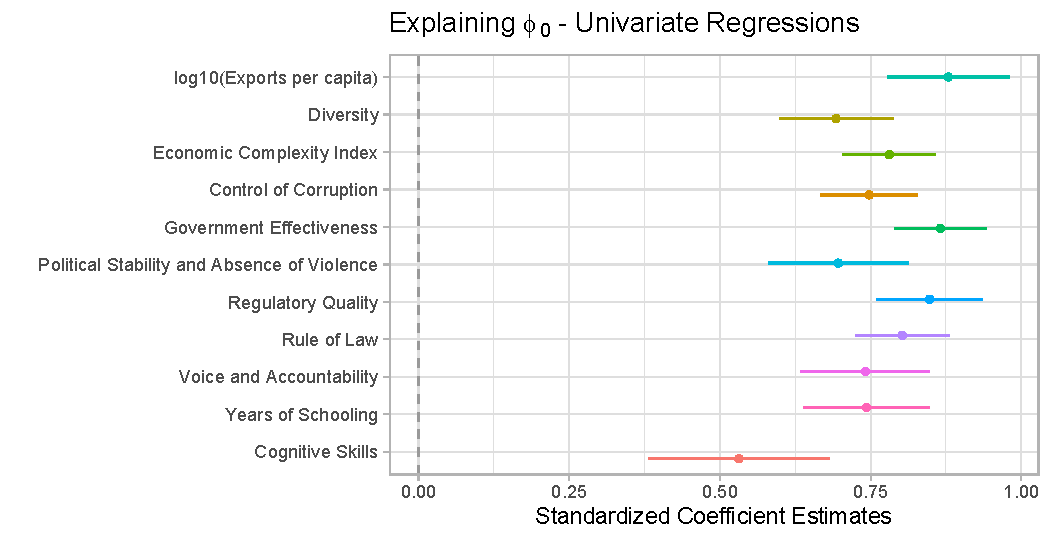
\includegraphics[width=0.7\columnwidth]{C:/Users/agomez/Dropbox/Identify laws and dynamical systems in socioeconomic data/machine_learned_patterns_in_economic_development/notebooks/regression_figures/PC0_regressions_coefficients_univariate.pdf}
\caption{
\textbf{Coefficients of the predictors from univariate regressions.} 
 All regressions included year-specific fixed-effects, errors are clustered by country and error bars reflect $95\%$ confidence intervals. The estimates are for standardized coefficients.}
\label{fig:regcoefs_univariate}
\end{center}
\end{figure}

\begin{figure}[htb]
\begin{center}
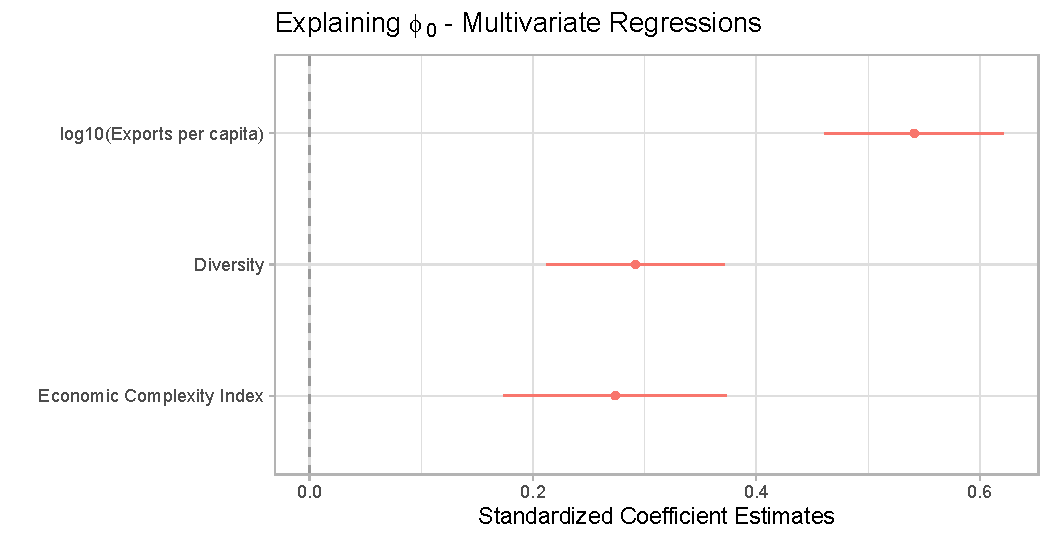
\includegraphics[width=0.7\columnwidth]{C:/Users/agomez/Dropbox/Identify laws and dynamical systems in socioeconomic data/machine_learned_patterns_in_economic_development/notebooks/regression_figures/PC0_regressions_coefficients_smallmultivariate.pdf}
\caption{
\textbf{Coefficients of the predictors from a multivariate regression only including exports per capita, diversity and economic complexity index.} 
 All regressions included year-specific fixed-effects, errors are clustered by country and error bars reflect $95\%$ confidence intervals. The estimates are for standardized coefficients.}
\label{fig:regcoefs_smallmultivariate}
\end{center}
\end{figure}

\begin{figure}[htb]
\begin{center}
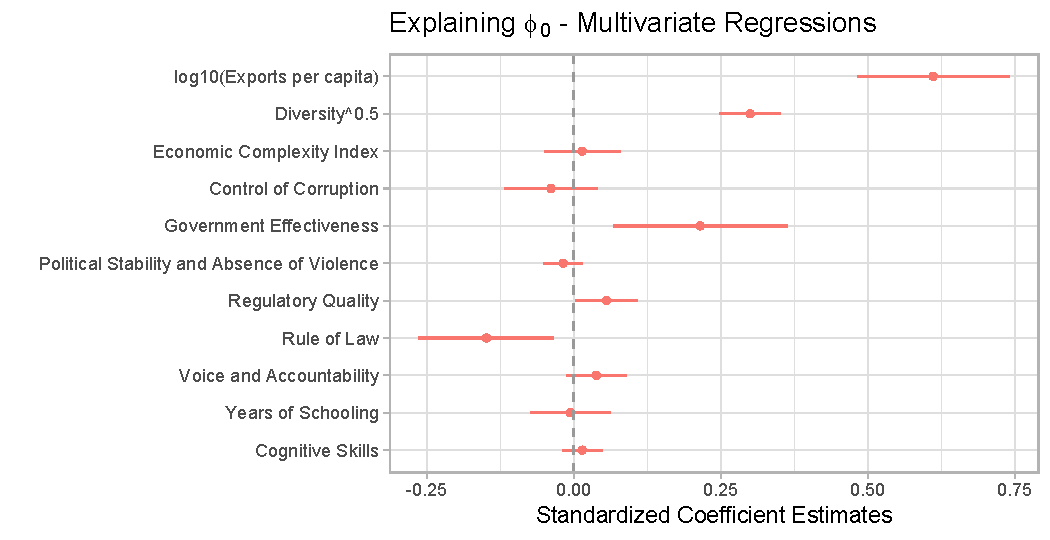
\includegraphics[width=0.7\columnwidth]{C:/Users/agomez/Dropbox/Identify laws and dynamical systems in socioeconomic data/machine_learned_patterns_in_economic_development/notebooks/regression_figures/PC0_regressions_coefficients_multivariate.pdf}
\caption{
\textbf{Coefficients of the predictors from a multivariate regression including.} 
 All regressions included year-specific fixed-effects, errors are clustered by country and error bars reflect $95\%$ confidence intervals. The estimates are for standardized coefficients.}
\label{fig:regcoefs_multivariate}
\end{center}
\end{figure}


\begin{figure}[htb]
\begin{center}
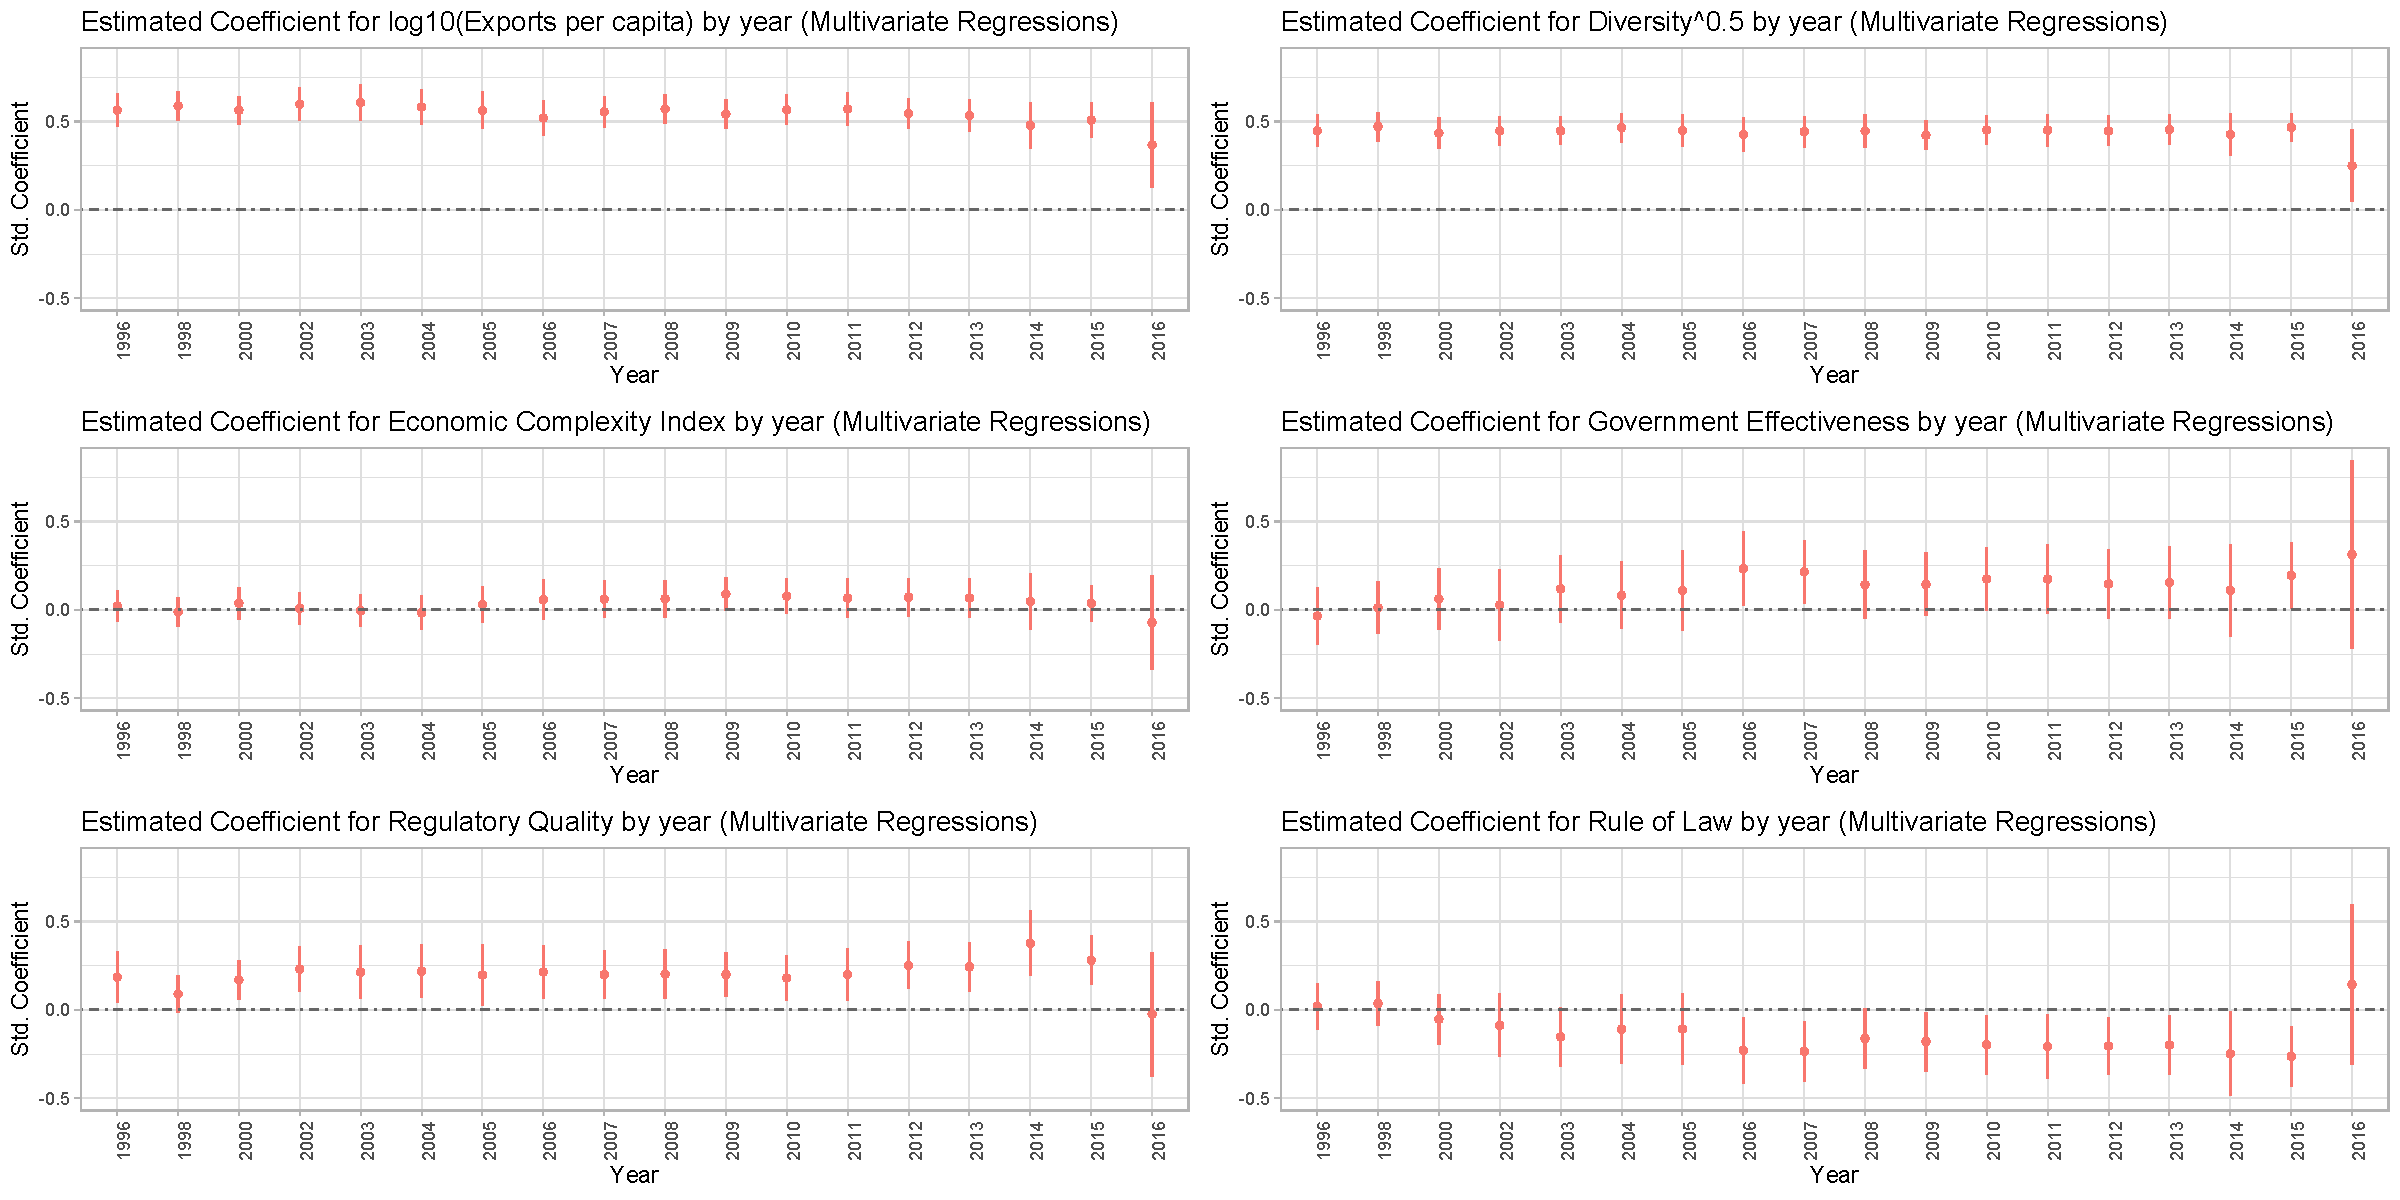
\includegraphics[width=\columnwidth]{C:/Users/agomez/Dropbox/Identify laws and dynamical systems in socioeconomic data/machine_learned_patterns_in_economic_development/notebooks/regression_figures/PC0_acrossyears_regressions_coefficients_subset_multivariate.pdf}
\caption{
\textbf{Coefficients of the predictors from multivariate regressions carried separately by year.} 
 The estimates are for standardized coefficients.}
\label{fig:regcoefs_acrossyears}
\end{center}
\end{figure}


As can be seen, while all regressors predict to some extent $\scoreFirstPC$ when we carry out univariate regressions, when all are put together only exports per capita, diversity, government effectiveness, and rule of law survive. In the multivariate regressions done per year, the coefficients for exports per capita and diversity are consistently significant and positive, and have similar magnitudes.
